84. а) $y=\cfrac{x^2-2x}{2-x}+4=\cfrac{x(x-2)}{2-x}+4=\begin{cases} 4-x,\\ x\neq 2.\end{cases}$\\
\begin{figure}[ht!]
\center{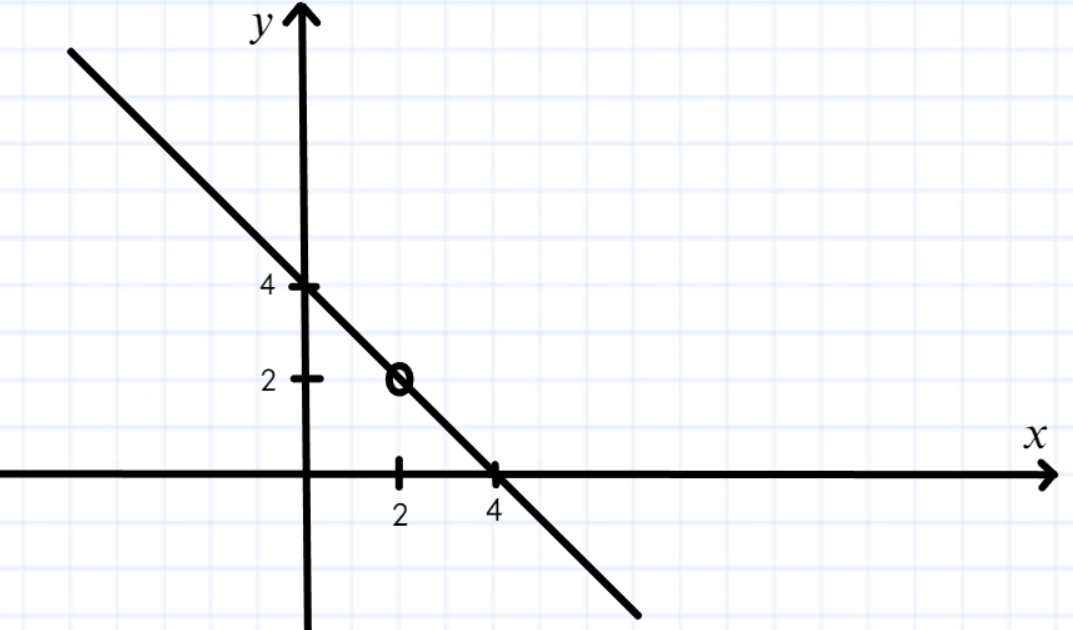
\includegraphics[scale=0.35]{gr7-84.png}}
\end{figure}\\
б) При положительных $x$ функция принимает значения $(-\infty;2)\cup(2;4).$\\
в) Эта прямая не будет иметь общих точек с графиком функции, если она параллельна прямой $y=4-x$ или если она проходит через выколотую точку $(2;2).$ Пусть это прямая $y=kx+b.$ В первом случае её угловой коэффициент равен $-1,$ значит $-1=-1+b,\ b=0,$ то есть это функция $y=-x.$ Во втором случае $\begin{cases} -1=k+b,\\ 2=2k+b.\end{cases}\Leftrightarrow
\begin{cases} -3=-k,\\ b=2-2k.\end{cases}\Leftrightarrow
\begin{cases} k=3,\\ b=-4.\end{cases},$ то есть прямая задана уравнением $y=3x-4.$\newpage\noindent
